\chapter{Fotometría}
La luz proveniente de los objetos astronómicos y que es recolectada por los telescopios, únicamente nos brinda información sobre la posición y movimiento de las fuentes en el cielo, su brillo aparente, líneas espectrales y la energía que emiten. A estas cantidades se les llama <<observables>>. A pesar de esta limitante, el ser humano ha comprendido mucho sobre las estrellas y las galaxias con ayuda de algunos principios físicos. Gracias a ello, es posible extraer más información de los observables, como la distancia a la fuente, luminosidad, temperatura, composición química, tamaño, campos magnéticos, velocidades. Aprenderemos un poco sobre cómo los astrónomos determinan estos parámetros en las siguientes dos clases.

\section{Conceptos de fotometría}
Las fuentes astronómicas se clasifican en puntuales y extensas. En la mayoría de los instrumentos, las estrellas aparecen como fuentes puntuales, mientras que las fuentes extensas incluyen objetos como nebulosas, galaxias y el fondo cósmico de microondas. El tratamiento de la luz de estos dos tipos de fuentes varía, y es responsabilidad de la \textbf{fotometría}, una rama de la óptica dedicada al estudio y la medición precisa de la luz.

Exploraremos el tema de la fotometría, comenzando por el sistema que los astrónomos utilizan para describir el brillo aparente de las estrellas, el cual, aunque fundamental, puede resultar bastante confuso y contraintuitivo.

\subsection{Sistema de magnitudes}
\subsubsection{Flujo y luminosidad}
Lo único que los telescopios son capaces de medir es la cantidad de fotones que llegan a la superficie del detector en un tiempo dado. Este parámetro se define como el flujo y lo representaremos con la letra $ F $, sus unidades son  $ \mathrm{ph~ cm^{-2} ~ s^{-1} }$ (fotones/unidad de área/unidad de tiempo). 

El flujo es una cantidad física que varía inversamente proporcional al cuadrado de la distancia. Esto significa que mientras más lejana sea la fuente, más pequeño será el flujo detectado. Esto se conoce como la ley del inverso del cuadrado y se ilustra de manera esquemática en la Figura \ref{fig:flux-inverse}, donde una fuente puntual está eemitiendo luz en todas las direcciones (isotrópicamente). La cantidad de luz que pasa a través de una superficie de área $A$ varía dependiendo de la distancia a la que se encuentra la superficie. 

\begin{figure}[htb]
  \centering
  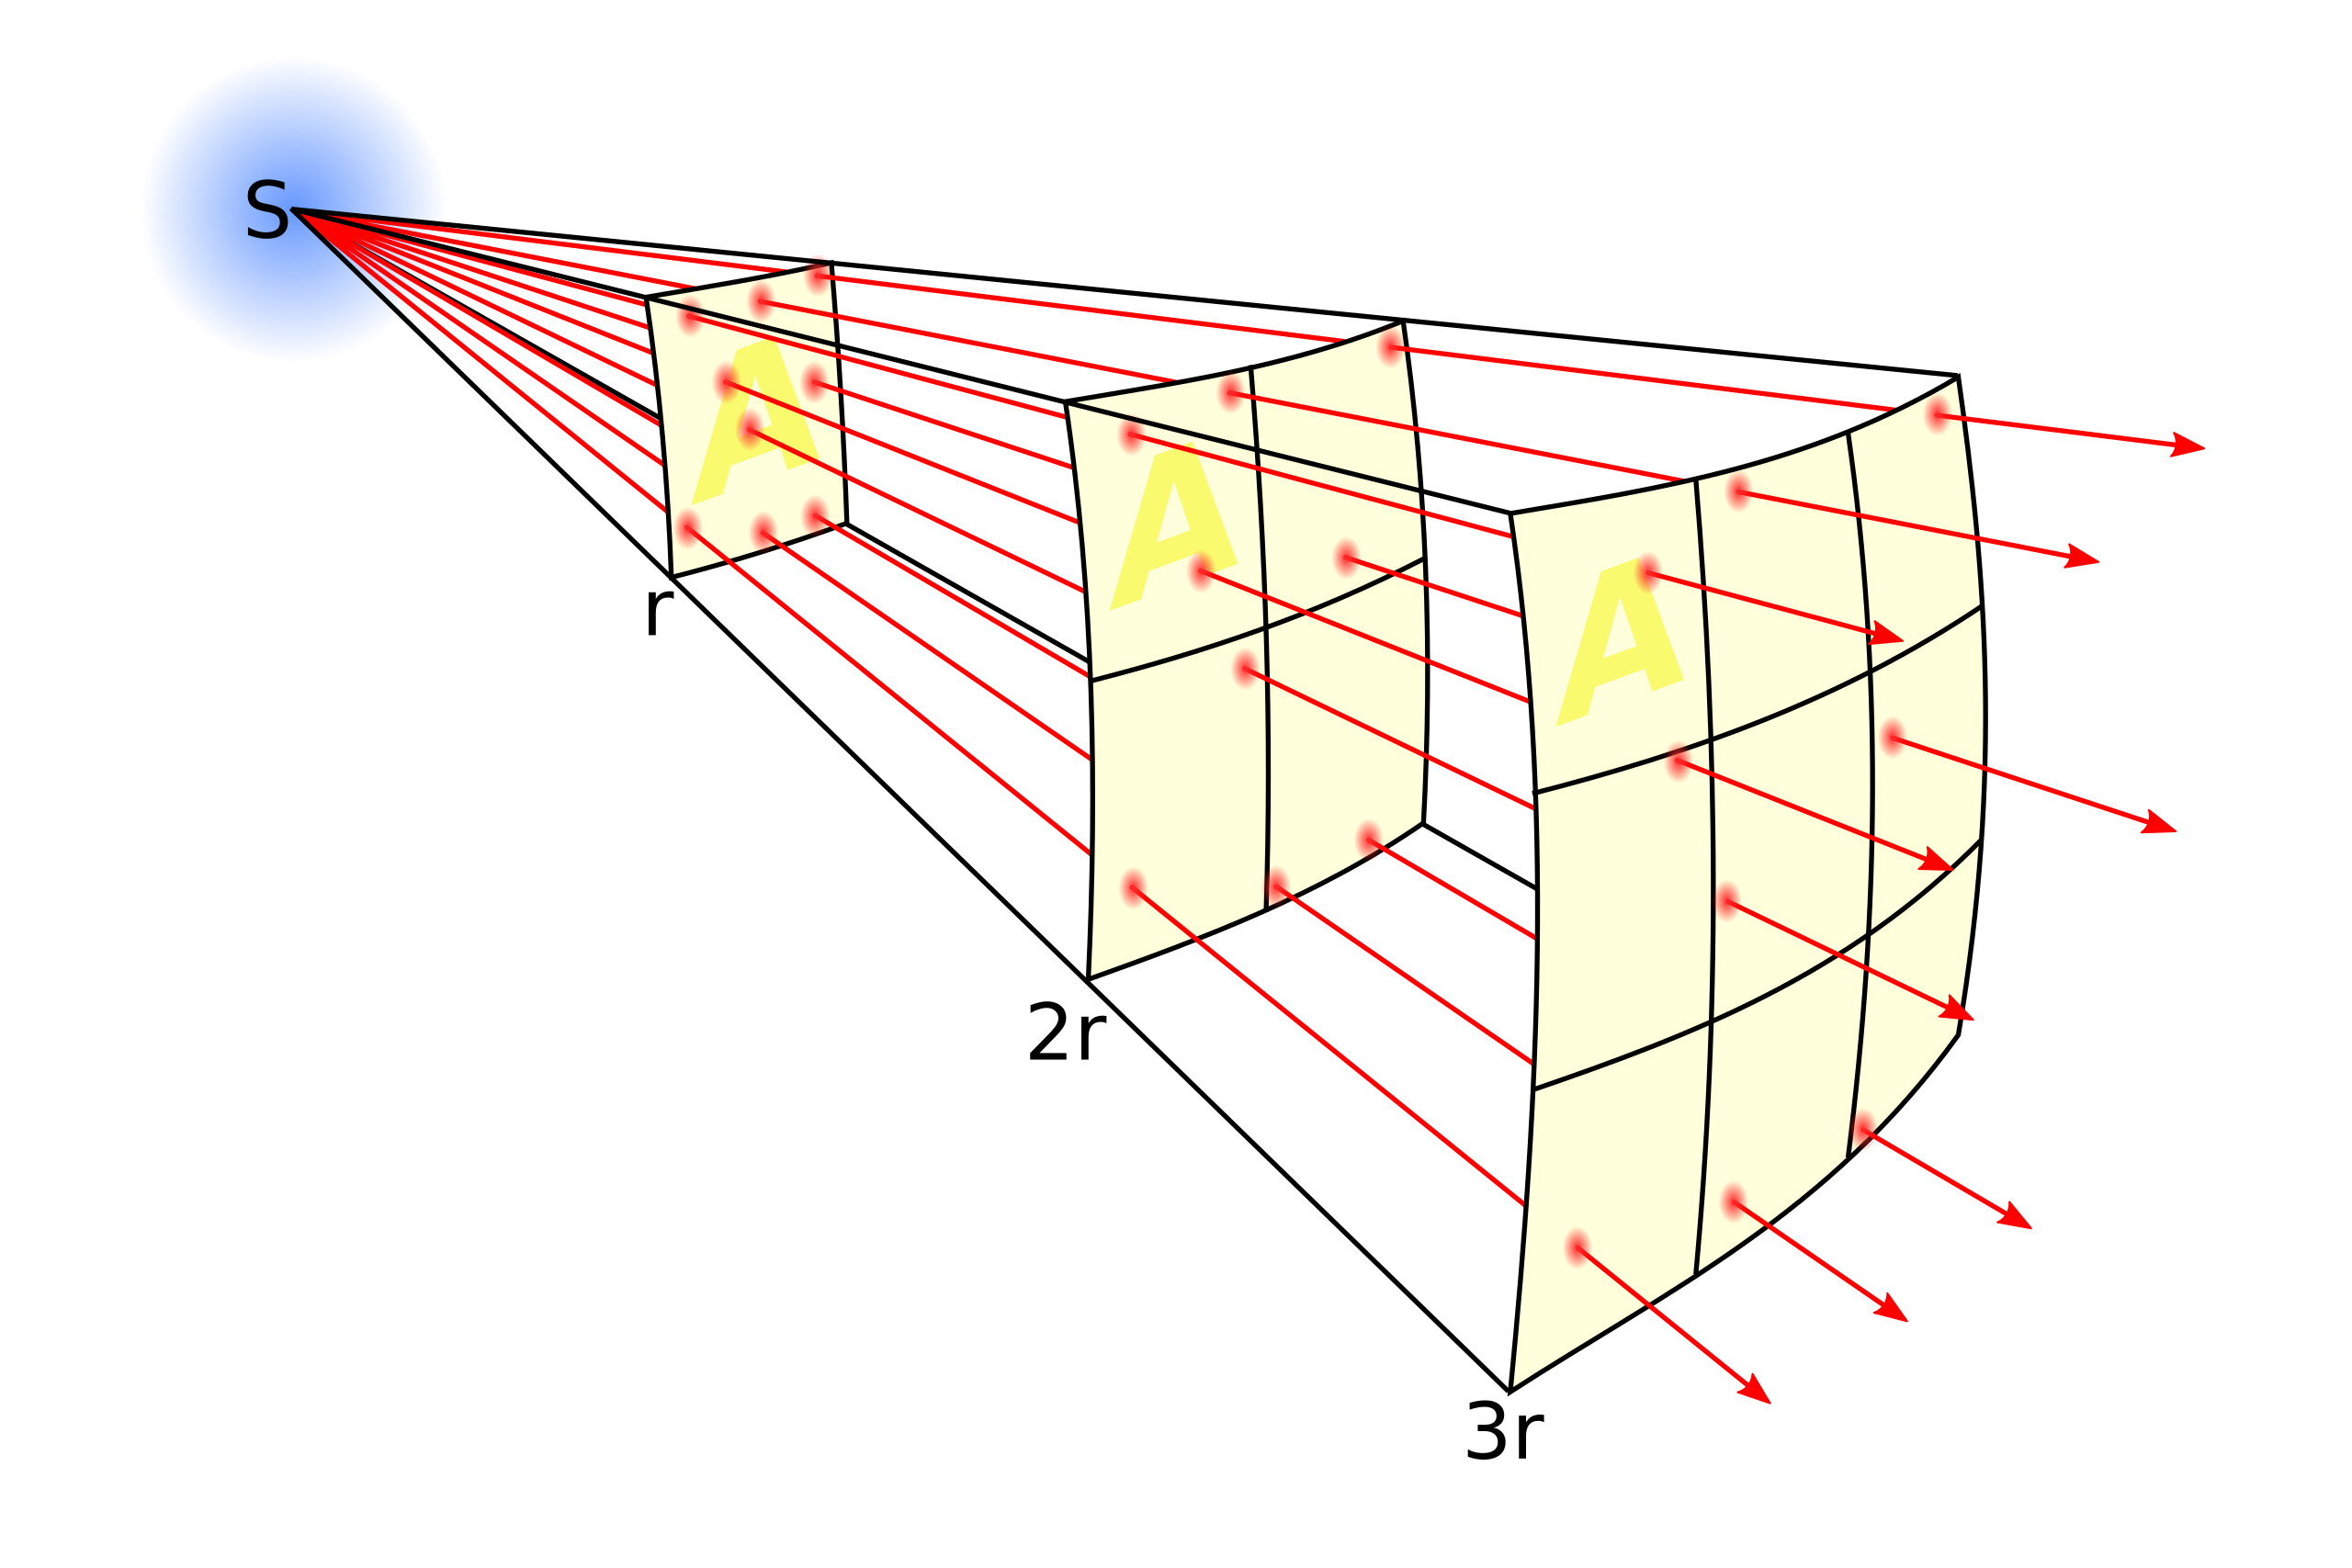
\includegraphics[width=0.8\textwidth]{figures/Inverse_square_law.png}
  \caption{Esquema de la ley del inverso del cuadrado para flujos}
  \label{fig:flux-inverse}
\end{figure}

Asumiendo que la luz de una fuente astronómica se distribuye de manera isotrópica, entonces a una distancia $ r $, el área superficial está dada por $ A_1 = 4\pi r^2 $ y el flujo será $ F_1 \propto \frac{1}{A_1} = \frac{1}{4\pi r^2} $. En cambio a una distancia igual a $ 2r $, el área estará dada por $ A_2 = 4\pi (2r)^2 = 16 \pi r^2 = 4A_1 $ y el flujo será $ F_2 \propto \frac{1}{4A_1}  = \frac{1}{4}F_1$. Por lo tanto, si se duplica la distancia de la fuente, el flujo disminuye en un factor de 4. 

La constante de proporcionalidad en $ F \propto 1/(4\pi r^2) $ es una cantidad muy importante llamada luminosidad. La luminosidad se define como la energía total liberada por una fuente astronómica, se denota con la letra $ L $ y su valor depende de las propiedades de cada estrella, pero no de la distancia. En otras palabras, la relación matemática entre el flujo y la luminosidad es:
\[ F = \frac{L}{4\pi r^2} \]
donde $ r $ es la distancia a la que se encuentra la fuente. Un parámetro muy importante es el valor del flujo en la superficie de la estrella. Si la estrella tiene un radio $ R $, entonces el flujo superficial, $ F_S $ está dado por:
\[ F_S = \frac{L}{4\pi R^2}. \]
Podemos resolver esta ecuación para la luminosidad y se obtiene:
\[ L = 4\pi R^2 F_S = AF_S, \]
esto nos permite estimar la luminosidad a partir de parámetros de la estrella como su radio $ R $ y su flujo superficial $ F_S $. Con ayuda de la termodinámica es posible demostrar que 
\[ F_S = \sigma T^4, \] 
donde $ \sigma = 5.67 \times 10^{-5} \mathrm{~erg ~ cm^{-2} ~ s^{-1} ~ K^{-4}} $ es la constante de Stefan-Boltzmann y $T$ es la temperatura en la superficie de la estrella, medida en kelvins ($\mathrm{K}$). Al combinar esta expresión con la luminosidad, se obtiene el resultado:
\[ L = A \sigma T^4, \]
el cual es conocido como la ley de Stefan-Boltzmann.

\subsubsection{Magnitudes}
El brillo de una estrella puede describirse mediante \textbf{magnitudes}, donde magnitudes más grandes corresponden a estrellas más tenues. El concepto de magnitud se utiliza desde los tiempos de Hiparco, quien dividió las estrellas visibles en seis grupos de magnitudes igualmente separadas de acuerdo al ojo humano. Las estrellas más brillantes fueron clasificadas como magnitud 1, mientras que las menos brillantes, de magnitud 6. Esta clasificación poco intuitiva se basó originalmente en la apariencia de las estrellas cuando comenzaba a oscurecer durante el ocaso. Aquellas estrellas que aparecían primero (por lo tanto, las más brillantes) se clasificaron como de magnitud  1, las segundas fueron clasificadas como de magnitud 2 y así sucesivamente hasta llegar a las de magnitud 6 (las últimas en aparecer eran las más tenues). Debido a que la clasificación se basa en criterios del ojo humano, se conocen como <<magnitudes aparentes>>.

Esta convención de magnitudes se sigue utilizando en la actualidad y se formula de la siguiente manera. La sensibilidad del ojo humano a la luz sigue una escala logarítmica, entonces definimos a $ m_1 $ y $ m_2 $ como las magnitudes aparentes de estrellas cuyos flujos son $ F_1 $ y $ F_2 $. Ya que estas cantidades deben seguir una escala logarítmica, se cumple la relación:
\[ m_1 - m_2 = -k \log\qty(\frac{F_1}{F_2}), \]
donde el signo negativo se utiliza para asignar los valores de magnitud más pequeños a las estrellas más brillantes. Diferentes estudios fotométricos indican que las estrellas de magnitud 6 son alrededor de 100 veces menos brillantes que las de magnitud 1. Matemáticamente se puede expresar como $F_1/F_2 = 100$ y además $m_1 - m_2 = 1-6 = -5 $. Con esto se encuentra que $k = 2.5$ y entonces la relación para magnitudes es:

\[ m_1 - m_2 = 2.5\log_{10}\left(\frac{F_1}{F_2} \right); \quad \frac{F_1}{F_2} = 10^{\frac{2}{5}(m_1 - m_2)}. \]

Algo muy importante que hay que resaltar de este resultado es que no es posible determinar la magnitud de una estrella por sí misma, solo se puede comparar con otra estrella y determinar la diferencia entre sus magnitudes. Además, la ecuación no define un <<punto cero>> o magnitud de punto cero de manera explícita, de modo que una forma más general es
\[ m = -2.5\log(F) + C, \]
donde $ C $ es el <<desfase>> del punto cero. 

Para que este sistema funcione, se debe definir una estrella de magnitud cero, llamada estrella estándar, con la cual sea posible comparar y obtener la magnitud de cualquier otra. De este modo, todos los astrónomos deben coincidir que cierta estrella tiene cierta magnitud. Debes tener en cuenta de que a pesar que se utilizan magnitudes para cuantificar el brillo de las estrellas, la cantidad medible u observable es en realidad el flujo. 

Las estrellas estándar comenzaron a definirse gracia a los avances en la fotometría fotográfica en los años 1950. Actualmente, la estrella estándar es Vega, que es del tipo espectral A0 (hablaremos de esto más adelante)Cálculos más modernos implican que la magnitud de Vega es en realidad $0.03$.

Una vez definidas las estrellas estándar, es posible obtener la magnitud de cualquier otra. Por ejemplo, la magnitud de Capella es de $0.1$ y la de Sirio es de $-1.6$. Los objetos más brillantes en el cielo son por supuesto la Luna y el Sol, debido a su cercanía y tienen magnitudes de $-12.5$ y $-26.76$, respectivamente. Algunas de las estrellas más tenues que se han observado gracias el Telescopio Espacial Hubble (HST, por sus siglas en inglés) tienen magnitudes de hasta $30.7$. 

\subsubsection{Magnitudes bolométricas y absolutas}
Todos los telescopios tienen un rango de longitudes de onda en los que son capaces de observar. En la práctica, las magnitudes se obtienen para una región específica del espectro electromagnético. Por ejemplo, cuando hablamos de magnitudes aparentes, nos referimos a magnitudes en el rango visible, pero también se trabaja en otras longitudes de onda. La versión \textbf{monocromática} (es decir, a una longitud de onda específica) de la relación entre magnitudes y flujos es:
\[ m_{\lambda} = -2.5 \log(F_{\lambda}) + C_{\lambda} \]

El extremo opuesto a la magnitud monocromática es la \textbf{magnitud bolométrica}, que para su medición incluye la radiación en todas las longitudes de onda emitidas por la fuente. Estas magnitudes se indican con el subíndice <<bol>> y es posible aplicar una corrección bolométrica (BC, por sus siglas en inglés) a cualquier medición, simplemente calculando la diferencia entre la magnitud bolométrica y la magnitud en cualquier otra banda de longitudes de onda (como la visual):
\[ BC_{\mathrm{bol}} = m_{\mathrm{bol}} - m_{\mathrm{band}} \]

Otra cantidad de importancia es la \textbf{magnitud absoluta}, la cual se define como la magnitud aparente que tendría una estrella si estuviera ubicada a $10 ~\mathrm{pc}$. Supongamos que el flujo de una estrella a una distancia $ d $ es $ F $. Si ahora colocamos esa misma estrella a una distancia $ d_0 $, entonces su flujo será $ F_0 $. Como se trata de la misma estrella, la luminosidad es la misma y entonces:
\[ L = 4\pi d_0^2 F_0 = 4\pi d^2 F,\]
de aquí se obtiene que
\[ \frac{F}{F_0} = \left( \frac{d_0}{d} \right)^2. \] 

Sea $ m $ la magnitud de la estrella a una distancia $ d $ y $ M $ su magnitud absoluta, es decir, a una distancia $ d_0 = 10 \mathrm{pc} $, entonces la relación entre $ m $ y $ M $ es la siguiente:
\[ m - M =  -2.5\log\left( \frac{F}{F_0} \right) = -2.5\log\left( \frac{d_0}{d} \right)^2 = 2.5 \log\left( \frac{d}{d_0} \right)^2 = 5 \log\left( \frac{d}{d_0} \right), \]
y sustituyendo $ d_0 = 10 \mathrm{pc} $:
\[ m - M = 5\log\left( \frac{d}{10pc} \right) = 5\log(d) - 5. \]

La cantidad $ m - M $ es conocida como el \textbf{módulo de distancia}. Para objetos que se encuentran a más de unos cuantos pársecs, la luz proveniente de ellos se dispersa con el medio interestelar y esto provoca que se vean más tenues. Este efecto se llama \textbf{extinción interestelar} y debe tomarse en cuenta. Por lo tanto, una relación más útil es la del \textbf{módulo de distancia aparente}:
\[ (m - M)_{\lambda} = 5\log(d) - 5 + A_{\lambda}, \]
donde $ A_{\lambda} $ es la absorción en magnitudes a una longitud de onda $ \lambda $.

Quizás la cantidad más importante de todas es la \textbf{magnitud bolométrica absoluta}, denotada por $ M_{\mathrm{bol}} $ que puede usarse para obtener la luminosidad de una estrella en términos de la luminosidad solar:
\[ M_{\mathrm{bol}} = 4.74 - 2.5\log\left( \frac{L}{L_{\odot}} \right), \]
donde $ L_{\odot} $ es la luminosidad solar y se mide en $ \mathrm{erg~s^{-1}} $.

\subsubsection{Índices de color}
Algunos detectores de luz son más sensibles en un rango específico de longitudes de onda. En otras palabras, si un detector en más sensible a longitudes de onda cortas, algunas estrellas podrían verse más azules en el detector comparadas al ojo humano. Por lo tanto, cuando se establece una magnitud, se debe especificar cómo fue determinada.

Esta diferencia en la sensibilidad permite determinar magnitudes en diferentes bandas de luz o energía, lo que da lugar a cuantificar el color de las estrellas. El \textbf{índice} de color se define como la diferencia entre las magnitudes de una estrella en dos bandas distintas. Normalmente, la banda visible se identifica con la letra $ B $, la banda ultravioleta con la letra $ U $ y la banda azul, con la letra $ B $. Así, el índice de color $ B - V $ de una estrella está dado por
\[ B - V = m_B - m_V, \]
donde $ m_B $ y $ m_V $ son las magnitudes en la banda ultravioleta y visible, respectivamente. Una estrella con $ B - V < 0 $ se ve más azul que una estrella con $ B - V > 0 $. 

\subsubsection{Filtros de color}
Es bastante común trabajar con filtros de color, los cuales son dispositivos que solo permiten  pasar luz con una longitud de onda específica. Uno de los sistemas de filtros más utilizados es el $ UBV $, el cual permite pasar luz únicamente en un rango estrecho de ultravioleta, azul y visible. La sensibilidad de este tipo de filtros se muestra en la Figura \ref{fig:filters-ubv}.

\begin{figure}[htb]
  \centering
				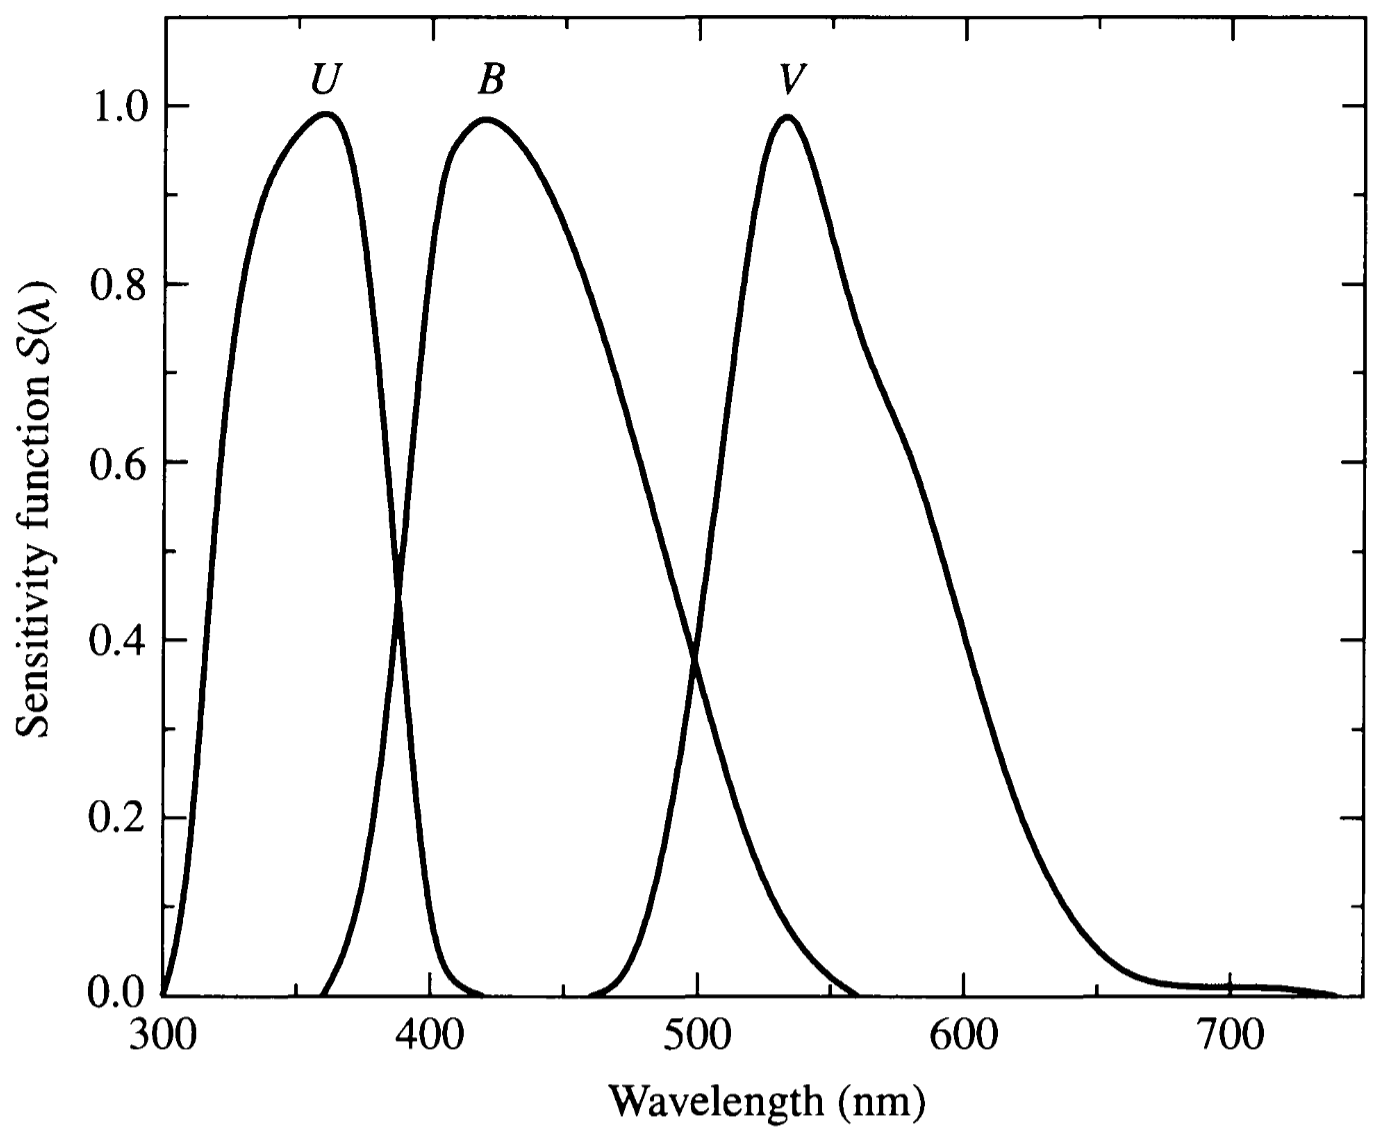
\includegraphics[width=\textwidth]{figures/UBV-filter.png}
				\caption{Curva de sensibilidad del ssitema de filtros $ UBV $.}
				\label{fig:filters-ubv} 
\end{figure}

Como se puede apreciar en la Figura \ref{fig:filters-ubv}, los filtros tienen una sensibilidad del $ 100\% $ en un intervalo muy estrello de longitudes de onda:
\begin{itemize}
  \item El filtro $U$ está en la región ultravioleta, centrado en $365 \mathrm{~nm}$ y con un espesor efectivo de $68~ \mathrm{nm}$.
  
  \item El filtro $B$ está en la región azul, centrado en $440 ~\mathrm{nm}$ y con un espesor efectivo de $98 ~\mathrm{nm}$
  
   \item El filtro $V$ está en la región visible, centrada en $550 \mathrm{~nm}$ y con un espesor efectivo de $89 ~\mathrm{nm}$​.
\end{itemize}

\subsection{Radiación de cuerpo negro}
En astronomía se utiliza el concepto de radiación electromagnética emitida por un objeto idealizado llamado \textbf{cuerpo negro}, que se define como un objeto que absorbe y emite luz de manera perfecta a todas las longitudes de onda. El flujo de un cuerpo negro depende solo de su temperatura superficial y está dado por las funciones de Planck:
\begin{align*}
  B_{\nu}(T) = \frac{2 h \nu^3}{c^2} \frac{1}{e^{h\nu/(kT) -1}} \\
  B_{\lambda}(T) = \frac{2hc^2}{\lambda^5}\frac{1}{e^{hc/(\lambda kT) -1},}
\end{align*}
donde las unidades son $ \mathrm{erg ~ s^{-1} ~ cm^{-2} Hz^{-1} ster^{-1}} $ en la primera ecuación y $ \mathrm{erg ~ s^{-1} ~ cm^{-2} cm^{-1} ster^{-1}} $ en la segunda. Los esteradianes (ster) son unidades de ángulo sólido; el cielo completo tiene $ 4\pi $ esteradianes. Una gráfica de esta distribución se muestra en la Figura \ref{fig:planck-function}.

\begin{figure}[htb]
  \centering
				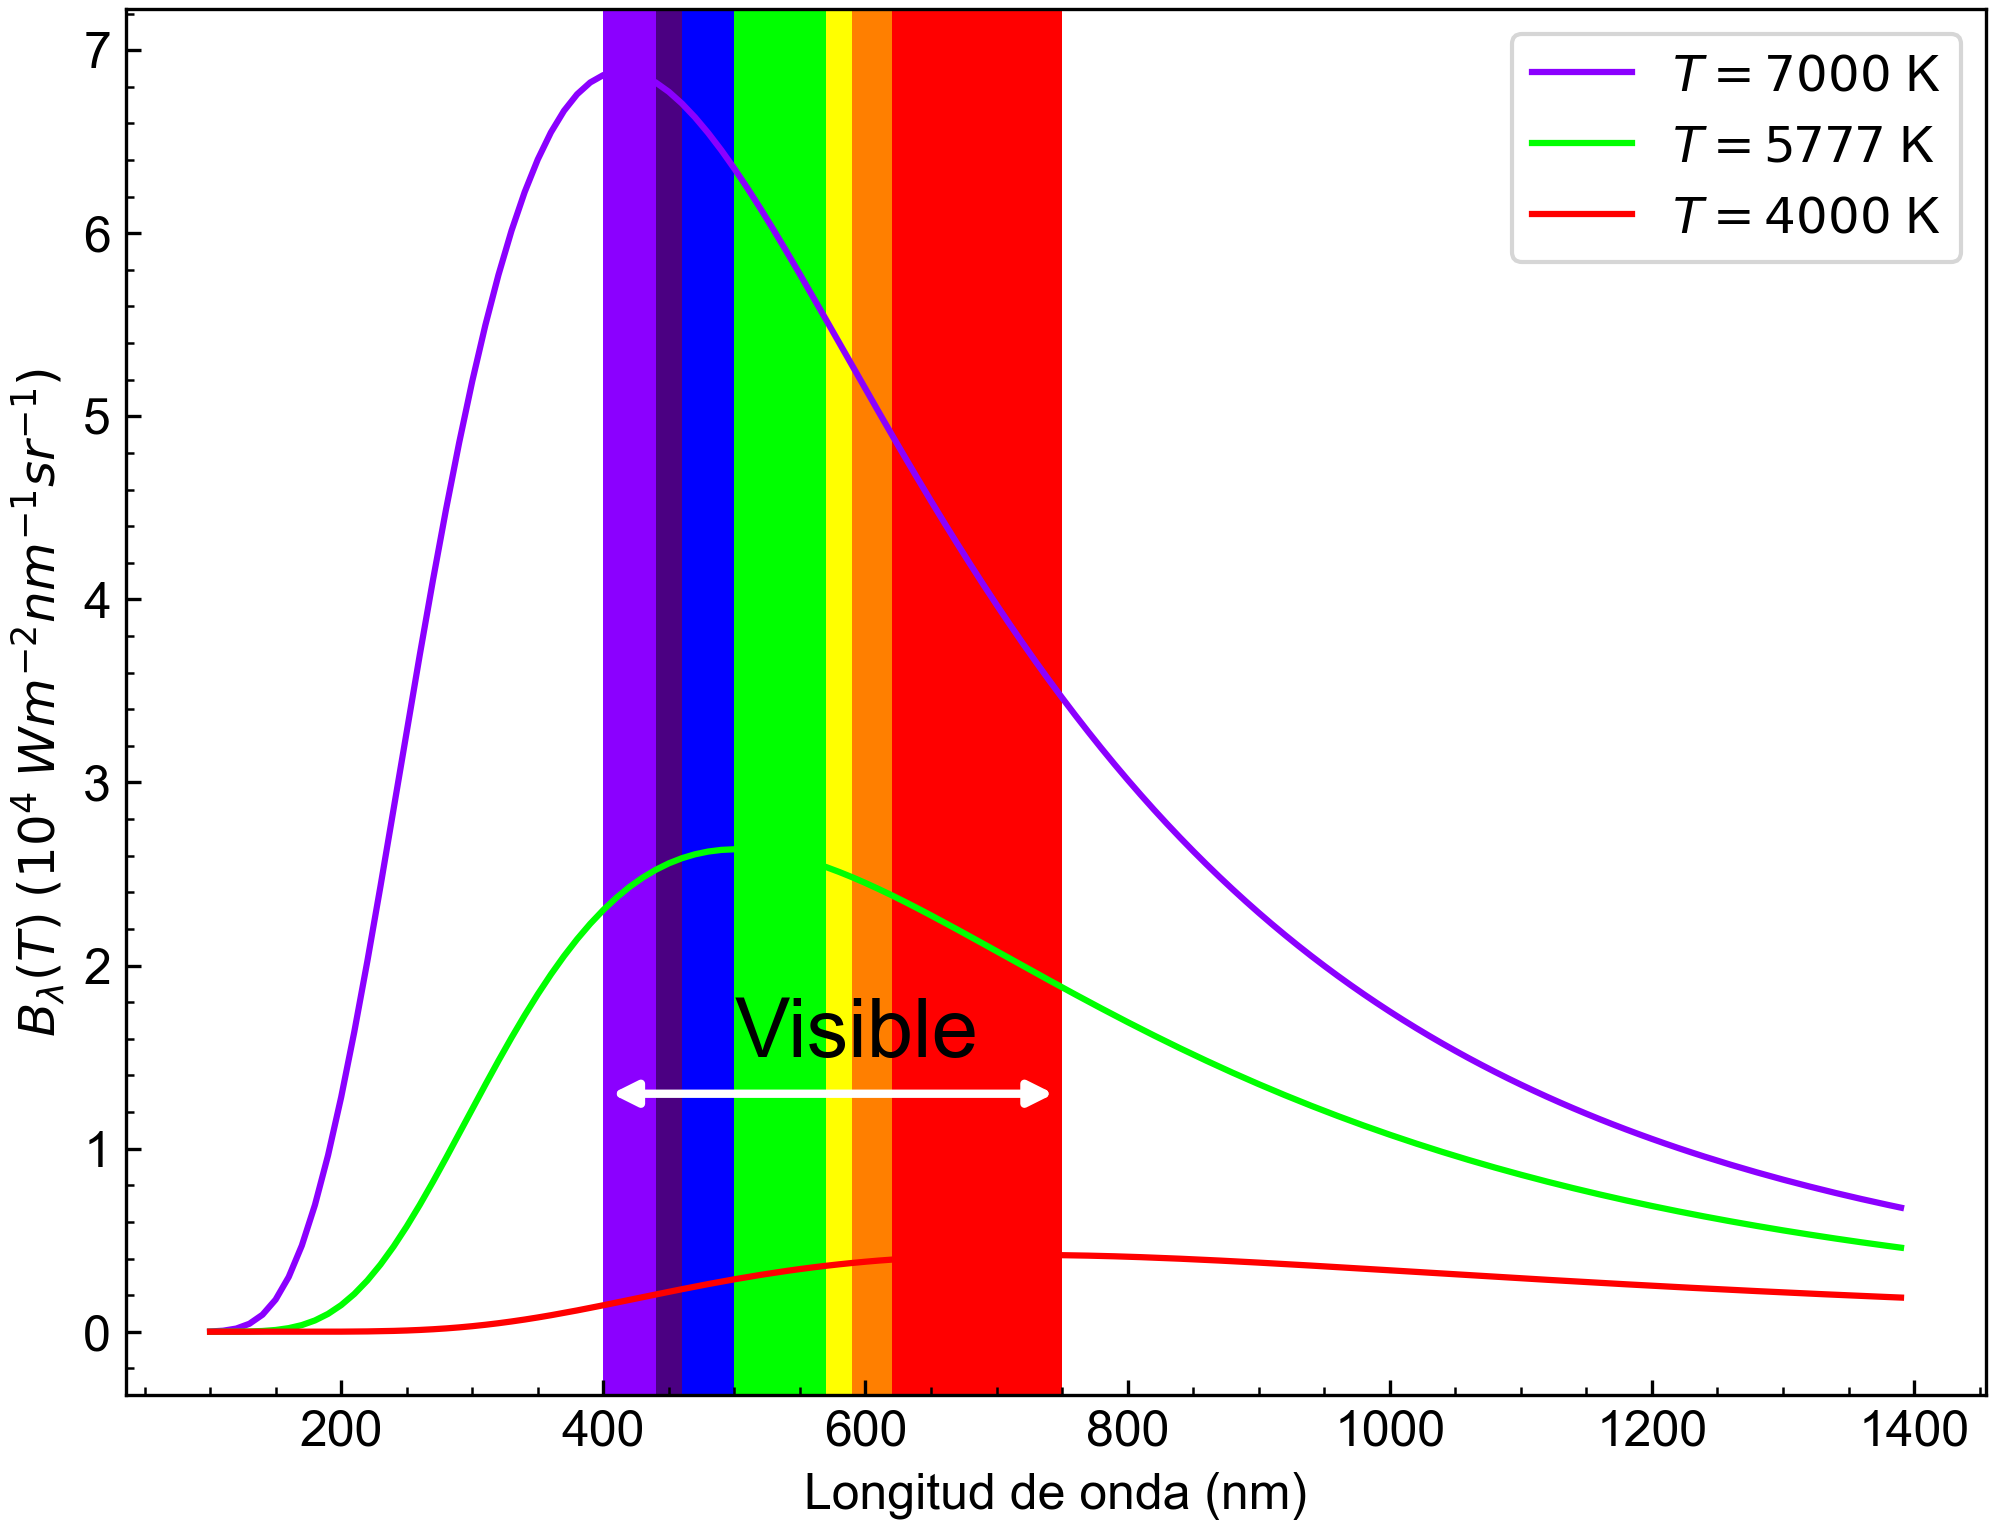
\includegraphics[width=\textwidth]{figures/Black_body.png}
				\caption{Distribución de energía de un cuerpo negro para diferentes temperaturas.}
				\label{fig:placnk-function} 
\end{figure}

La ley de desplazamiento de Wien nos ayuda a obtener la longitud de onda a la que ocurre el máximo de cada distribución en función de la temperatura:
\[ \lambda_{\mathrm{\max}} = \frac{c}{T}, \]
donde $ c = 2900000 \mathrm{K ~ nm} $ y la temperatura se mide en $ \mathrm{K} $. 
